\documentclass[conference]{IEEEtran}

\usepackage[utf8]{inputenc}
\usepackage[T1]{fontenc}
\usepackage{silence}\WarningsOff[latexfont]

\usepackage{amsmath}

\RequirePackage{tikz}[2010/10/13]
\usetikzlibrary{arrows,automata,calc,intersections,patterns,decorations.pathmorphing,decorations.pathreplacing}

\usepackage{graphicx}
\usepackage{cite}
\usepackage{url}
\usepackage[caption=false,font=footnotesize]{subfig}
\usepackage[binary-units,per-mode=symbol]{siunitx}
\sisetup{list-final-separator = {, and }}
\usepackage{booktabs}
\usepackage{pifont}
\usepackage{microtype}
\usepackage{textcomp}
\usepackage[american]{babel}
\usepackage[noabbrev,capitalise]{cleveref}
\usepackage{xspace}
\usepackage{hyphenat}
\usepackage[draft,inline,nomargin,index]{fixme}
\fxsetup{theme=color}
\usepackage{grffile}
\usepackage{xfrac}
\usepackage{multirow}
\RequirePackage{xstring}
\RequirePackage{xparse}
\RequirePackage[index=true]{acro}
\NewDocumentCommand\acrodef{mO{#1}mG{}}{\DeclareAcronym{#1}{short={#2}, long={#3}, #4}}
\NewDocumentCommand\acused{m}{\acuse{#1}}
\usepackage{upquote}

\acrodef{WSN}{Wireless Sensor Network}
\acrodef{MANET}{Mobile Ad Hoc Network}
\acrodef{ROI}{Region of Interest}{short-indefinite={an}, long-plural-form={Regions of Interest}}

\begin{document}

\title{Characterization of a population parameters}

\author{
	\IEEEauthorblockN{Rodrigo Joni Sestari, Mat. number 179020}
	\texttt{rodrigo.sestari@unitn.it}
}

\maketitle

\begin{abstract}
This document describes the work to estimates parameters from a dataset affected by noise and it also introduces a sinusoidal bias
\end{abstract}

\acresetall

\section{Introduction}
\label{sec:introduction}

\begin{itemize}
\item An electronic probe measures the output of a circuitry, which is known to generate i.i.d. samples \begin{math} y_i \end{math} taken from a population with a logistic distribution. 
\bigskip
\begin{center}\begin{math} x_i = A\sin\left(2\pi ft \right) + Y  +Z;  \ i =1,...60,000 \end{math}  \\
where: \begin{math} Y \sim  Logis(\mu,s) \ Z \sim N(0,\sigma_{n} )\end{math}  \end{center}
\bigskip
\item problem: how  estimates of \begin{math}
	A, f , \mu , s, \sigma_n
\end{math} and to evaluate the confidence interval of \begin{math}
	 \hat{\mu}
\end{math}   which is the most important parameter for the characterization of the circuitry.
\bigskip
\item strategy: the parameters come solved one by one,  using the knowledge you already have. Probing is done with a frequency of 20 kHz, and the measure lasts 3s, so that the sample contains 60,000 points.
\bigskip
\item assumption: X is Gaussian noise with zero mean and \begin{math} \sigma_{n} \end{math}; the frequency is a integer value.
\end{itemize}
\bigskip


\section{Implementation}

\begin{itemize}

\item  The first parameter to be evaluate is the \begin{math} \mu \end{math}. Knowing that the media of Z is zero and the mean of sinusoids is zero, then the mean of Y is the mean of dataset, in this case \begin{math} \mu = 2.003023 \end{math}. 
\bigskip
\item  The next parameter to be evaluate is the sinusoid frequency, but to discovery it, is necessary firstly discovery the the sinusoid points, knowing sinusoid points, we need just divide the the dataset points by sinusoid points and then, divide the result by measure time. To discovery how main points is compose a sinusoid we can use the auto correlation: \begin{math} COV(X_i(t + \tau), X_j(\tau))\end{math}. In the Figure 1, is possible see the autocorrelation dataset, the sinusoid is composed by 32 points, so the frequency of a sinusoid is \begin{math}
(60.000points/32points)/3s = 625 Hz  \end{math} then the parameter \begin{math} f=625Hz\end{math}.
\bigskip
\item Having the sinusoid frequency, the next parameter to be evaluate is the sinusoid Amplitude. The sinusoid Amplitude is estimate through the Regression Trigonometric, but first to apply this function was created a new dataset without the Logistic mean, the sinusoidal mean from each 32 points was extracted from this new dataset, the regression function was applied in the sinusoidal mean. The regression coefficient will be the sinusoid amplitude. In the Figure 2, is possible see the sinusoid Fit, the function coefficient is \begin{math} A = 1.772977\end{math}. Having the Amplitude and Frequency sinusoidal, is possible remove the sinusoid from the dataset, to be free to concentrate in the next to parameters  \begin{math} s, \sigma_n \end{math}
\bigskip
\item Is necessary some algebric steps to estimate \begin{math} s, \sigma_n \end{math}. Is possible estimate these two parameters using the Kurtosis function, we know that the excess kurtosis for a logistic distribution is \begin{math} \frac{6}{5} \end{math}, and for the normal distributions is 0. The Variance and Kurtosis was extracted from the dataset without the sinusoidal bias.  The first parameter to be estimate is \( \sigma_n \): 
\bigskip
	\\ Assumption:
	 \begin{math} 
 		\\
		\kappa_y =  \frac{6}{5}  \\
 		\kappa_z = 0 \\
	    \sigma_y^2 =  t \\
	    var \left( x_y + x_z \right)  =   \upsilon  \\
	    \upsilon  =  \sigma_y^2 + \sigma_z^2 \\
	    \sigma_z^2 =  \upsilon -\sigma_y^2 \\
	    \sigma_z^2 =  \upsilon -t \\
	    kurt\left( x_y + x_z \right) - 3= 0.4796231 \\
	    kurt\left( x_y + x_z \right) = \kappa    
	    \\	 
	  \end{math} 	  
	  \\Kurtosis functions:\\   
	  \begin{math}   
		kurt\left( x_y + x_z \right) -3 = \left( \frac{  {\sigma_y^4}* \left( \kappa_y -3 \right) 
		+{\sigma_z^4}* \left( \kappa_z -3 \right) }
       {\left(  {\sigma_y^2} + {\sigma_z^2} \right)^2 }\right)  \\
kurt\left( x_y + x_z \right) -3 = \left(
 \frac{- \frac{9 }{5}   {\sigma_y^4} -3{\sigma_z^4}  } 
      { \left({\sigma_y^2} + {\sigma_z^2} \right)^2}
\right) \\
-3 \left( v - {\sigma_y^2}  \right)^2  - \frac{9}{5}   {\sigma_y^4} =  \left(  \kappa -3\right) \upsilon ^2  \\
-3 \left(  \upsilon   -t  \right)^2 - \frac{9}{5} t^2   =  \left(  \kappa -3\right) \upsilon^2  \\
-3 \left( \upsilon^2 -2   \upsilon  t + t^2   \right) -\frac{9}{5} t^2 =  \left( \kappa -3\right) \upsilon^2  \\
-3 \upsilon^2 +6 \upsilon  t -3 t^2 -\frac{9}{5} t^2  =  \left( \kappa -3\right) \upsilon^2  \\
 -\frac{24}{5}  t^2 +6 \upsilon  t -3 \upsilon^2 -\left( \kappa -3\right) \upsilon^2 = 0 \\ 
  \end{math} 	  
	  \\Using the quadratic equations:\\   
	  \begin{math}  
t_1,t_2 =\frac{-b\pm\sqrt{b^2-4ac}}{2a} \\
  \end{math} 	  
	  \\Where:\\   
	  \begin{math}  
a=-\frac{24}{5}, \ \ b=+6 \upsilon ,\ \ c=-3 \upsilon^2 -\left( \kappa -3\right) \upsilon^2 \\
\end{math} 	  
	  \\Then:\\   
	  \begin{math}  
t_1=2.819502,   \sigma_z^2_1 = 30.01755\\
t_2=38.22682,   \sigma_z^2_2 = -5.389762\\
\end{math} 
\\by definition the variance can not be negative, then \begin{math} \sigma_n \end{math} is: \( \sqrt{30.01755}=5.478828 \)
\bigskip

\item The process to calculate  \( s \) is similar: \\ \\ Assumption:
	 \begin{math} 
 		\\
 		\sigma_y^2 =  v -\sigma_z^2 \\
	    var \left( x_y + x_z \right)  = 32.83706 \\
	  \end{math} 	  
	  
	  \\Then:\\   
	  \begin{math}  
 \sigma_y^2_1 = v - \sigma_z^2_1 =  32.83706 -30.01755 = 2.819502\\
   \sigma_y^2_2 =v - \sigma_z^2_2 = 32.83706 +5.389762 = 38.22682 \\
\end{math} 
	  \\The relation between variance and \( \sigma_n \) is:
	  \\
\begin{math}  
s^2 =  \frac{\sigma_y^2*3}{\pi^2} \\
\end{math} 
	 \\Then:\\  
\begin{math}  
s_1 =\sqrt{\left( \frac{2.819502*3}{9.869604} \right)} = 0.9257569 \\
s_2 =\sqrt{\left( \frac{38.22682*3}{9.869604}\right)} = 3.408747 \\
\end{math} 

\\
\item The last parameter to be estimate is the confidence interval for \begin{math} \hat{\mu}\end{math}. The CI is given by \begin{math} \left( \overline{X} -  \frac{ Z_\frac{\alpha}{2} *\sigma}{\sqrt{n}} \right) ,\mu, \left( \overline{X} +  \frac{ Z_\frac{\alpha}{2} *\sigma}{\sqrt{n}} \right) \end{math}. To calculate the interval confidence, was used the batch approach, totalising 75 subsets. Applying the CI  
\begin{math} \left(  2.003023 \pm  \frac{ 1.96 *0.1890665}{\sqrt{75}} \right) 
\end{math}, is possible affirmative with \begin{math} 95\% \end{math} that the mean is between  \begin{math} [1.960233,2.045813]\end{math}.
\end{itemize}

\bigskip
\section{Conclusion}

The objective this document was explain how estimate of \begin{math} A, f , \mu , s, \sigma_n
\end{math} and to evaluate the confidence interval of \begin{math}
	 \hat{\mu}
\end{math}. The parameter \begin{math} \hat{\mu}=2.003023 \end{math} was found knowing that the mean of Gaussian and Sinusoidal was zero. The sinusoid frequency \begin{math}  f = 625 Hz \end{math} was found through the autocorrelation, instead it amplitude \begin{math}  A = 1.772977 \end{math} through regression coefficient. the parameters \begin{math} s_1=0.9257569 \ s_2=3.408747 \ \sigma_n=5.478828 \end{math} was found using kurtosis function, and finally the CI of \begin{math} \hat{\mu}=[1.960233,2.045813] \end{math}. 


\section{Appendix}

   \begin{figure}
	\centering
	\subfloat{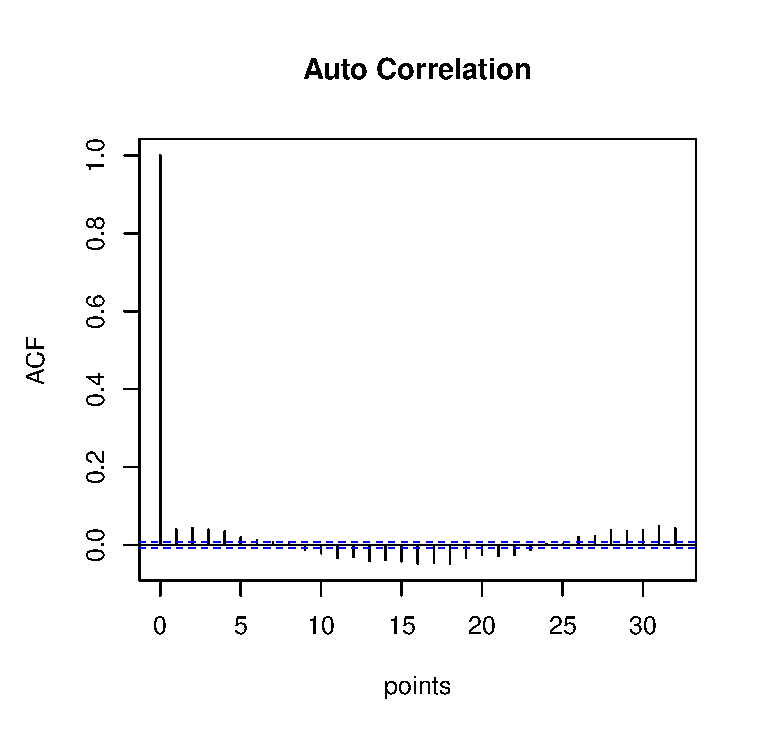
\includegraphics[width=\columnwidth]{figures/acf.eps}}
	\caption{The autocorrelation functions used to discovery the sinusoidal dimension.}%
  
	\subfloat{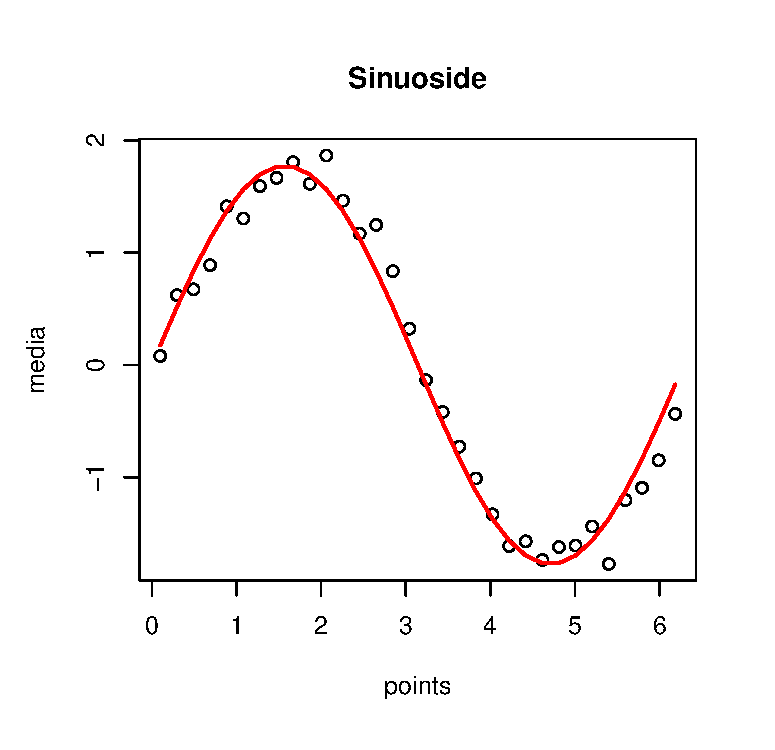
\includegraphics[width=\columnwidth]{figures/sinu.eps}}
	\caption{Sinusoid regression function, used to discovery the sinusoid amplitude}%
   \end{figure}


\end{document}



